% Search for all the places that say "PUT SOMETHING HERE".

\documentclass[11pt]{article}
\usepackage{amsmath,textcomp,amssymb,geometry,graphicx,enumerate}

\def\Name{Ran Liao}  % Your name
\def\SID{3034504227}  % Your student ID number
\def\Homework{3} % Number of Homework
\def\Session{Spring 2019}


\title{CS161--Spring 2019 --- Project \Homework\ Writeup}
\author{\Name, SID \SID}
\markboth{CS161--\Session\  Homework \Homework\ \Name}{CS161--\Session\ Project \Homework\ \Name}
\pagestyle{myheadings}
\date{\today}

\newenvironment{qparts}{\begin{enumerate}[{(}a{)}]}{\end{enumerate}}
\def\endproofmark{$\Box$}
\newenvironment{proof}{\par{\bf Proof}:}{\endproofmark\smallskip}

\textheight=9in
\textwidth=6.5in
\topmargin=-.75in
\oddsidemargin=0.25in
\evensidemargin=0.25in


\begin{document}
\maketitle

\section{Weaponize Vulnerability}
\begin{qparts}
	\item \textbf{Steal Dirks's Session ID}
	
	There's SQL injection vulnerability in server.py line 158.
	
	database.execute("UPDATE users SET \textbf{age=\{\}} WHERE username='\{\}';".format(age, username))

	The age parameter is not surrounded by single quote properly. Therefore, it's possible to inject malicious SQL codes here.
	
	Suppose age is \textbf{(SELECT id FROM sessions WHERE username="dirks")}.
	
	A subquery will be constructed and age will be changed to dirks's session id.
	
	\begin{figure}[h]
	\centering
	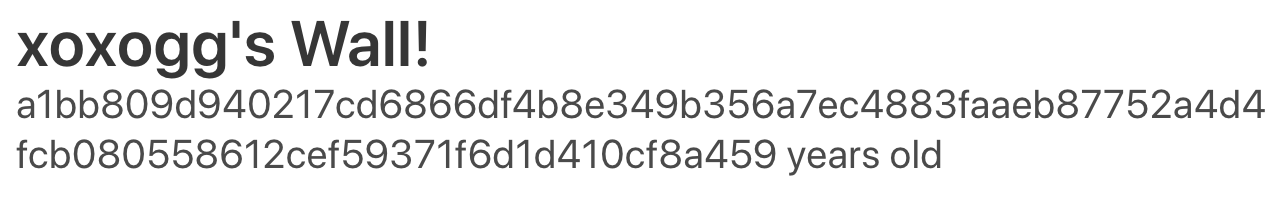
\includegraphics[width=0.5\textwidth]{session_id.png}
	\end{figure}
	
	\item \textbf{Log in through Dirks's Session ID}
	
	The server identify user by their session id. Therefore, if I modify my session id in cookies and set it to be dirks's session id. I can log in as dirks!
	
	This can be done either modify cookie directly through a chrome extension(EditThisCookie). Also, it's possible to use XSS attack to inject some script codes and modify cookies. For example, user can create a post like this 
	
	\textbf{\textless script\textgreater  document.cookie ="SESSION\_ID=a1bb809d940217cd6866df4b8e349b35 6a7ec4883faaeb87752a4d4fcb080558612cef59371f6d1d410cf8a459";\textless script\textgreater}
	
	\item \textbf{Create a Post as Dirks}
	(You can do whatever you want after you logged in as dirks.)
	\begin{figure}[h]
	\centering
	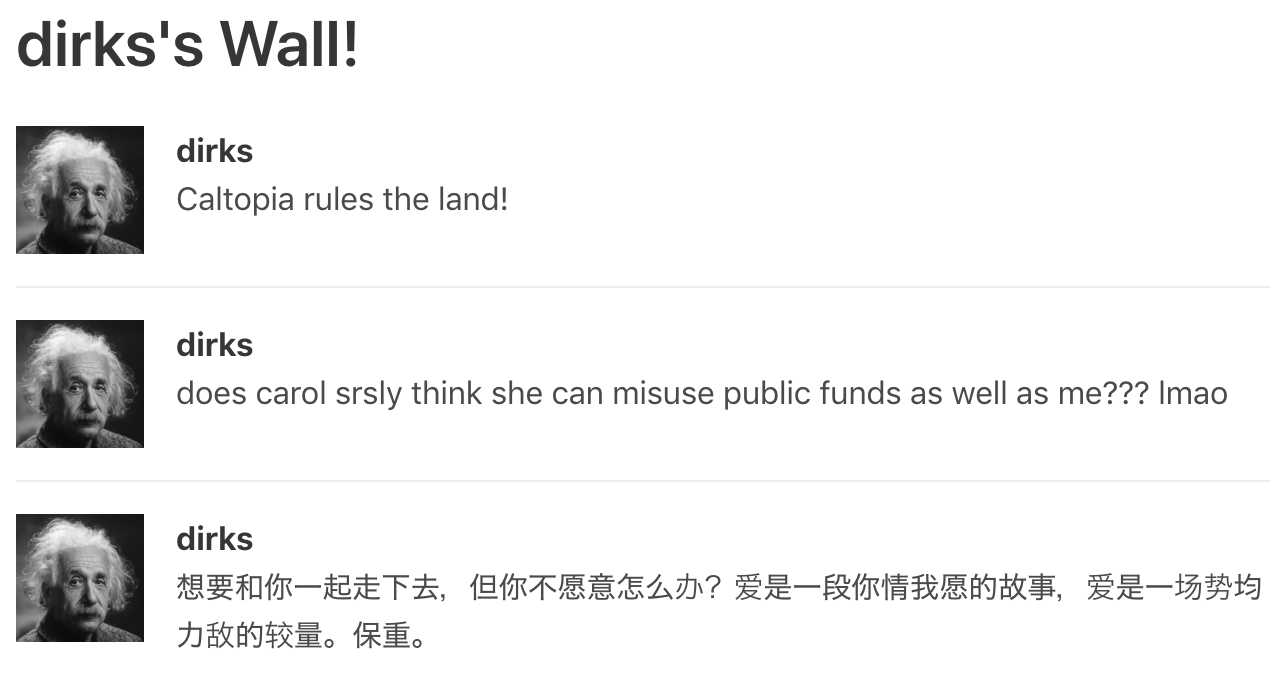
\includegraphics[width=0.5\textwidth]{post.png}
	\end{figure}
	
\end{qparts}

\newpage
\section{Vulnerability Writeup}
\begin{qparts}
	\item \textbf{Test 1}
	
	In server.py line 129, the buggy program do not validate the input username and echo it back directly. Therefore, the attacker can initiate a reflected XSS attack here.
	
	return render\_template('no\_wall.html', username=\textbf{other\_username})
	
	The attacker can visit a page like this
	
	http://127.0.0.1:5000/wall/\textbf{\textless body onload=alert("Reflected\_XSS")\textgreater}
	
	The last component of this url will be interpreted as javascript codes and will be executed automatically. The attacker can steal lots of sensitive information through this. i.e. user's cookie.
	
	It can be fixed by this
	
	return render\_template('no\_wall.html', username=\textbf{escape\_html(other\_username)})
	
	In general, we should validate every input gathered from user before using it. Sanitize input is a good idea. What's more, enable auto escape protection in Jinja template will be very helpful.
	
	\item \textbf{Test 5}
	
	In auth\_helper.py line 20, the buggy program do not sanitize session id before construct a sql query. Therefore, the attacker can inject sql statement here.
	
	found\_session = database.fetchone("SELECT username FROM sessions WHERE id='\{\}';".format(session))
	
	The attacker can give a malicious id like this, \textbf{' OR username='dirks}
	
	So the following query will be constructed. 
	
	\textbf{SELECT username FROM sessions WHERE id='' OR username='dirks';}
	
	Obviously, the attacker can bypass password protection and logged in as dirks.
	
	To fix it, just need to escape session id before constructing the statement.
	
	\textbf{session = escape\_sql(session)}
	
	In general, we can use prepared statement to construct sql query. The standard library will sanitize input properly.
	
	\item \textbf{Test 6}
	
	In server.py line 177, the buggy use \textbf{in} operator to validate user input, which is not sufficient.
	
	\textbf{if user\_dir \text{in} avatar:}
	
	The attacker can by pass this by giving input like this, \textbf{avatar\_images/xoxogg/../dirks/dirks.jpg}
	
	By exploiting this, the attacker can delete dirks's avatar image.
	
	The following code will fix this bug.
	
	\textbf{if user\_dir.startswith(os.path.realpath(avatar)):}
	
	In general, we can use \textbf{os.path.realpath} to get rid of all \textbf{.} and \textbf{..}.

\end{qparts}


\newpage
\section{Other Issues}
\begin{qparts}
	
	\item \textbf{Session ID Never Expire}
	
	User's session id is valid forever. This can cause huge problem. Actually, as I mentioned above, the attacker can use dirks's session id to bypass password protection. But if the session will expire, the risk will be much lower even if we don't fix those vulnerabilities.
	
	\item \textbf{Age Validation}
	
	Before update database, the server should check whether age is valid. In logic, an age should be an integer between 1 and 100. Check this before constructing sql statement will prevent potential sql injection effectively.
	
	\item \textbf{File Size Not Constrainted}
	
	The server doesn't check the size of avatar file before storing it. This could make server be vulnerable to DoS attack. To fix it, the server should deny all large files(maybe 100KB will be enough for an avatar).
	
	\item \textbf{Hide Internal Error / Do Error Handling}
	
	When I upload a file with invalid extension(not .jpg nor .jpeg), I will receive an HTTP 500 Internal Server Error. This is an error caused by server.py line 151.
	
	\textbf{stored\_avatar\_filename = avatar\_helper.save\_avatar\_image(avatar, username)}
	
	\textbf{stored\_avatar\_filename} will be \textbf{None} in this situation. The server doesn't check if before using it.
	
	Actually, the server should handle this error more properly. In general, HTTP 500 Internal Server Error should be hided and never be exposed to user or attacker.
	
	\item \textbf{Duplicate Avatar Filename}
	
	If I upload different avatars with same filename, the last version avatar will override the former one. This is not what user expected. The server could generate a random filename each time when received an avatar.


\end{qparts}







\end{document}